\section{Redes Neuronales Artificiales: Perceptrón Multicapa y Retropropagación}
\label{sec:u2_redes_neuronales}
La Unidad 2 profundiza en los modelos teóricos y técnicas algorítmicas de la minería de datos moderna.
\subsection{Fundamentación Teórica}
Análisis formal de las arquitecturas algorítmicas y criterios de convergencia e impureza.
\begin{figure}[H]
\centering
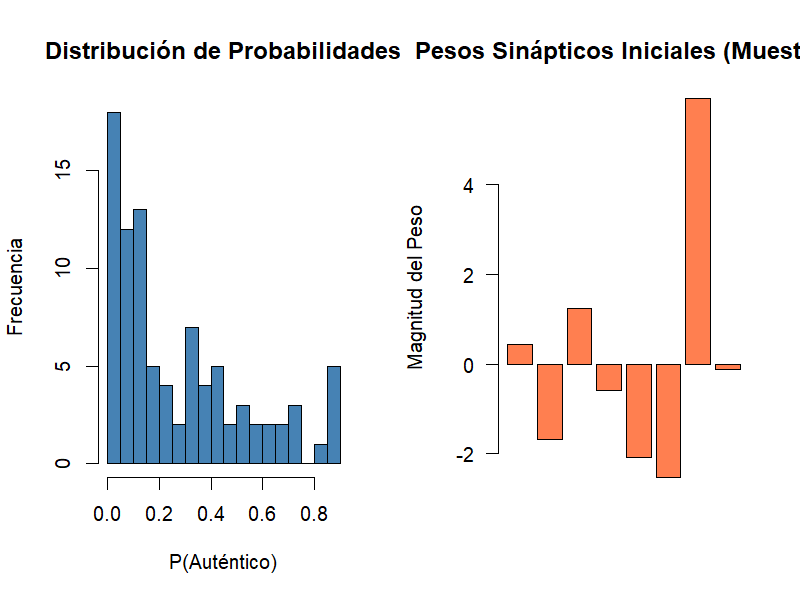
\includegraphics[width=0.82\textwidth]{figuras/grafico_04_red_neuronal.png}
\caption{Distribución de probabilidades y pesos en la Red Neuronal (MLP)}
\label{fig:u2_nn}
\end{figure}
\subsection{Conclusiones del Módulo}
La integración de estos métodos conforma la base analítica para la resolución de problemas predictivos complejos.
